\section{实验结果}

\subsection{生成图像与读取方式}

图~\ref{fig:input-pair} 展示程序实际使用的左右输入图像；图~\ref{fig:stereo-results}
从左至右给出归一化视差图、有效区域掩码和相对深度可视化。所有图片均直接引用
\codepath{task2/results/} 下的程序输出。图像只用于观察空间结构，定量结论来自
\codepath{disparity_raw.npy} 和 \codepath{depth_proxy.npy}。

\begin{figure}[H]
  \centering
  
\includegraphics[width=0.48\linewidth]{../results/left.png}\hfill
  
\includegraphics[width=0.48\linewidth]{../results/right.png}
  \caption{OpenCV 官方 aloe 双目输入图（左：\texttt{aloeL.jpg}，右：\texttt{aloeR.jpg}）。}
  \label{fig:input-pair}
\end{figure}

\begin{figure}[H]
  \centering
  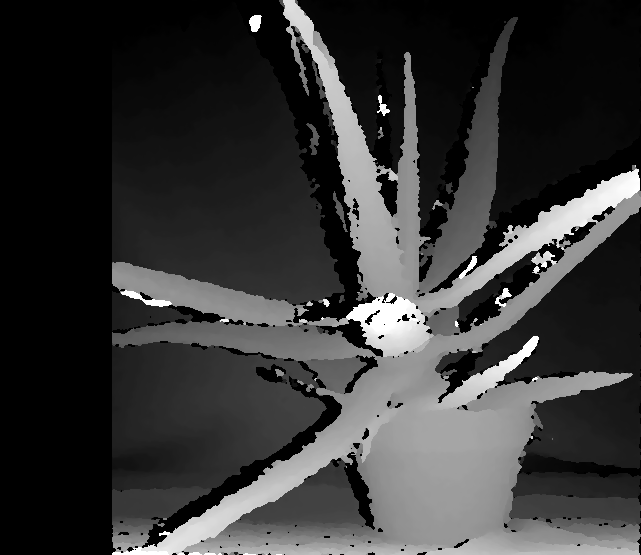
\includegraphics[width=0.31\linewidth]{../results/disparity.png}\hfill
  
\includegraphics[width=0.31\linewidth]{../results/valid_mask.png}\hfill
  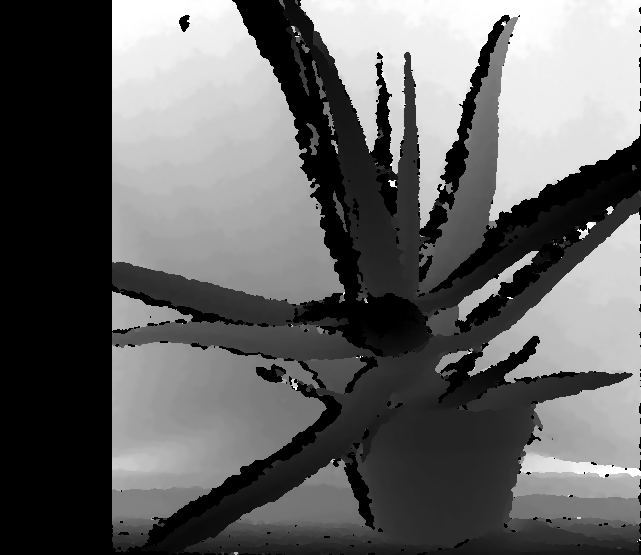
\includegraphics[width=0.31\linewidth]{../results/depth_proxy.png}
  \caption{程序生成的结果图（从左至右）：归一化视差图、有效视差掩码和任意尺度相对深度图。}
  \label{fig:stereo-results}
\end{figure}

归一化 PNG 通过百分位范围增强显示对比度，不能把 PNG 中的灰度数值直接代入
$Z=fB/d$。例如，某像素的真实视差应从 \codepath{disparity_raw.npy} 读取；相对深度应从
\codepath{depth_proxy.npy} 读取，二者都保留无效区域的 \texttt{NaN} 语义。

\subsection{真实运行结果}

统计直接读取程序生成的浮点数组，数组尺寸为 $555\times641$，总像素数为 $355755$。
在有限且满足 $d>15$ 的视差像素中，有 $261378$ 个有效像素，占总像素的
$73.4713\%$。表~\ref{tab:result-statistics} 汇总了真实运行结果。

\begin{table}[H]
  \centering
  \caption{OpenCV aloe 样例的真实运行结果统计}
  \label{tab:result-statistics}
  \begin{tabular}{ll}
    \toprule
    指标 & 实测值 \\
    \midrule
    原始图像尺寸 & $1282\times1110$ \\
    匹配图像尺寸 & $641\times555$ \\
    浮点数组尺寸 & $555\times641$ \\
    总像素 & $355755$ \\
    有效视差像素 & $261378$ \\
    无效像素比例 & $26.5287\%$ \\
    有效视差像素比例 & $73.4713\%$ \\
    有效视差范围 & $16.000$--$105.875$~px \\
    相对深度范围 & $0.0094451$--$0.0625$（任意尺度） \\
    公式核验误差 $\max|z-1/d|$ & $0.0$ \\
    \bottomrule
  \end{tabular}
\end{table}

\subsection{近远关系的定量解释}

将有效视差按数值排序后，较低的 0--5\% 区间为 $16.000$--$23.750$~px，其相对深度
代理中位数为 $0.043127$；较高的 95--100\% 区间为 $65.750$--$105.875$~px，其
相对深度代理中位数为 $0.014172$。后者小于前者，符合 $1/d$ 的单调关系，即较大
视差对应相对更近的区域。

视差图和相对深度图保留了叶片、花盆和背景的主要结构，说明固定参数的 StereoSGBM
已经产生有效匹配。有效掩码中的空白区域不是“零深度”，而是程序拒绝参与统计的
无效匹配。

\subsection{结果边界}

无效区域可能来自遮挡、纹理不足、重复纹理或左右图像边界处的搜索范围不足。它们不应
被填成任意数值来提高图像完整度。\texttt{aloeGT.png} 如被使用，只能作为官方视差参考图，
不能作为相机标定或米制深度真值。由于当前 aloe 图像对缺少经核验的 $f$、$B$ 和
$\mathbf{Q}$，本实验不能输出米、厘米等物理单位的绝对深度或带物理尺度的三维点云。
